\documentclass[oneside,9pt]{memoir}

% Colors
\usepackage[dvipsnames]{xcolor}

% hyperref
\usepackage[%
    colorlinks=true,
    linktocpage=true,
    breaklinks=true,
    linkcolor=RoyalBlue,
    urlcolor=RoyalBlue,
    citecolor=RoyalBlue
]{hyperref}
\def\sectionautorefname{§}


% Fonts
\usepackage{fontspec}
\setmainfont[Numbers = {OldStyle, Proportional}]{TeX Gyre Pagella}

%\usepackage{amssymb}
\usepackage{unicode-math}
\setmathfont{TeX Gyre Pagella Math}

% Typography
\usepackage[tracking]{microtype}

% Images
\usepackage{graphicx}

% ======================================================================
% Memoir package - layout and styling
% ======================================================================

% The calc package is required for calculating readable text widths
\usepackage{calc}

\DeclareMathOperator*{\argmax}{arg\,max}

% Set outer and spine margins A wide right margin is chosen both for legibility
% of the typeblock and for tight integration of marginfigures and margin
% footnotes.

% Calculate widths in pts
\setlxvchars[\normalfont\normalsize] % about 66 characters per column
\setxlvchars[\normalfont\footnotesize] % about 45 characters per column

% Set left and right margins
\setlrmarginsandblock{1.15in}{3.5in}{*}
% Set upper and lower margins
\setulmarginsandblock{1.1in}{1.1in}{*}

% Set properties of margin notes, sidecaptioned floats, and footnotes in the
% margin.
\setmarginnotes{0.2in}{2.15in}{2\onelineskip}
\setsidecaps{0.2in}{2.15in}
\sidecapmargin{outer}
\renewcommand*{\sidecapstyle}{\normalfont\footnotesize}
\setsidecappos{c}


% Set footnotes in the margin rather than at the foot of the page
\footnotesinmargin
\setsidefeet{\marginparsep}{1.9in}{0.2in}{0pt}{\flushleftright\footnotesize}{*}

% Integrate the counters of the sidefootnotes and footnotes in margin.
\letcountercounter{sidefootnote}{footnote}
\setlength{\footmarkwidth}{0em}
\setlength{\footmarksep}{-\footmarkwidth}
\setlength{\footparindent}{1em}
\sideparmargin{outer}

\renewcommand*{\sideparfont}{\color{Maroon}\emphshape}
\renewcommand*{\sideparvshift}{2\baselineskip}
\marginparmargin{outer}

% Style the entries in the Table of Contents
\renewcommand*{\cftchapterfont}{\scshape\MakeTextLowercase}
\renewcommand*{\cftpartfont}{\color{Maroon}\scshape\MakeTextLowercase}
\captionstyle[\centering]{\footnotesize}
\captionnamefont{\footnotesize\color{Maroon}}

%% Bringhurst chapter and head styles with a Pedersen-type chapter number
\makechapterstyle{bringhurst}{%
	\renewcommand{\chapterheadstart}{} 
	\renewcommand{\printchaptername}{} 
	\renewcommand{\chapternamenum}{} 
	\setlength{\midchapskip}{15mm}
	\renewcommand*{\printchapternum}{%
        \begin{marginfigure}[0pt]
          \resizebox{!}{\midchapskip}{\color{Maroon}\emph{\thechapter}}
        \end{marginfigure}
      }
	\renewcommand{\afterchapternum}{} 
	\renewcommand{\printchaptertitle}[1]{%
	  \raggedright\Large\scshape\MakeLowercase{##1}}
	\renewcommand{\afterchaptertitle}{%
	  \vskip\onelineskip \hrule\vskip\onelineskip}
}
\setlength{\cftsubsectionindent}{0.6in}
\chapterstyle{bringhurst}
\headstyles{bringhurst}

\tightlists

% Headers and footers - page numbers, section headings, etc.
\makepagestyle{tufte}
\createmark{chapter}{left}{nonumber}{}{}
\makeoddhead{tufte}{}{}{\scshape\MakeTextLowercase{\leftmark}~~|~~\thepage}
\makeevenhead{tufte}{\thepage~~|~~\scshape\MakeTextLowercase{\rightmark}}{}{}
 \makerunningwidth{tufte}[8in]{8in}
\aliaspagestyle{chapter}{empty}
\nouppercaseheads
\pagestyle{tufte}

\checkandfixthelayout

% Bibliography management
\usepackage[%
    style=authoryear-comp,
    natbib
]{biblatex}
\addbibresource{bibliography.bib}

% ======================================================================
% Creating the title page
% ======================================================================

\begin{document}
\begin{center}
    {\LARGE ToMCAT Study 3 Preregistration}\\
    \bigskip
    \textbf{Authors}
\end{center}

\begin{tabular}{ll}
    \toprule
    Name & Institution \\\midrule
    Salena Ashton & University of Arizona\\
    Loren Champlin & University of Arizona\\
    John Culnan & University of Arizona\\
    Kobus Barnard & University of Arizona\\
    Emily Butler & University of Arizona\\
    Ruihong Huang & Texas A\&M University \\
    Meghavarshini Krishnaswamy & University of Arizona\\
    Clayton Morrison & University of Arizona\\
    Md Messal Monem & Texas A\&M University \\
    Remo Nitschke & University of Arizona\\
    Adarsh Pyarelal & University of Arizona\\
    Ayesha Qamar & Texas A\&M University \\
    Adam Ussishkin& University of Arizona\\
    Yuwei Wang & University of Arizona\\
    Andrew Wedel & University of Arizona\\
    Liang Zhang & University of Arizona\\
    \bottomrule
\end{tabular}

\bigskip

\tableofcontents* 

\chapter{Introduction}
\textbf{Adarsh Pyarelal}

\section{Purpose and structure}

This document serves the following purposes.

\begin{itemize}
    \item Declare the capabilities we aim to demonstrate for our online agent
        components in ASIST Study 3
    \item Declare in advance -- with as much specificity as we can muster --
        the offline analyses we plan to perform on ASIST study 3 data.
\end{itemize}


The goal of the preregistration process as originally devised is to separate
hypothesis-generating (exploratory) research from hypothesis-testing
(confirmatory) research. A large portion of the activities engaged in by TA1
performers in ASIST - e.g., development of models, algorithms, and systems -
does not fit neatly into the paradigm of hypothesis generation and testing.
For this reason, while we endeavor to specify our analyses and capabilities in
as much detail as we can, we do not specify specific social science style
hypotheses to be tested\footnote{Whether TA1 performers \emph{should} be
specifying formal, quantitative hypotheses is another discussion.}.

The primary motivation for the structure of this preregistration document
is to accelerate the writing up of manuscripts for publication by using the
structure provided by the preregistration process to plan ahead for
publications.

Each of the sections in this document is a `component preregistation' that
corresponds to a publication `seedling', with the content optimized for what we
call `copy-pasteability', that is, the ability to be copied verbatim into a
manuscript for publication with minimal changes. This is intended to reduce
duplicate effort between writing up preregistrations and publications.

Since we are a fairly large team, each section has the names of the primary
authors responsible for the content of the section displayed under the section
heading. Authorship is ascribed to those who have contributed substantially to
the ideation or writing of the content.

\section{Overview}

Broadly speaking, we are aiming to develop a suite of open-source technologies
for artificial social intelligence, with a focus on computational understanding
of spoken team dialogue. Each of the component preregistrations demonstrates a
capability that we believe is important for artificial social intelligence, and
is currently integrated or will be integrated in the near future into our ASI
agent that will be evaluated in ASIST study 3 or future ASIST experiments.

\begin{itemize}
    \item Describe the architecture of the ToMCAT ASI and ACs. Provide one or
        more architecture diagrams.
    \item Give a brief summary of the preregistrations and how they contribute
        to the overall architecture.
\end{itemize}

\begin{figure}
    \centering
    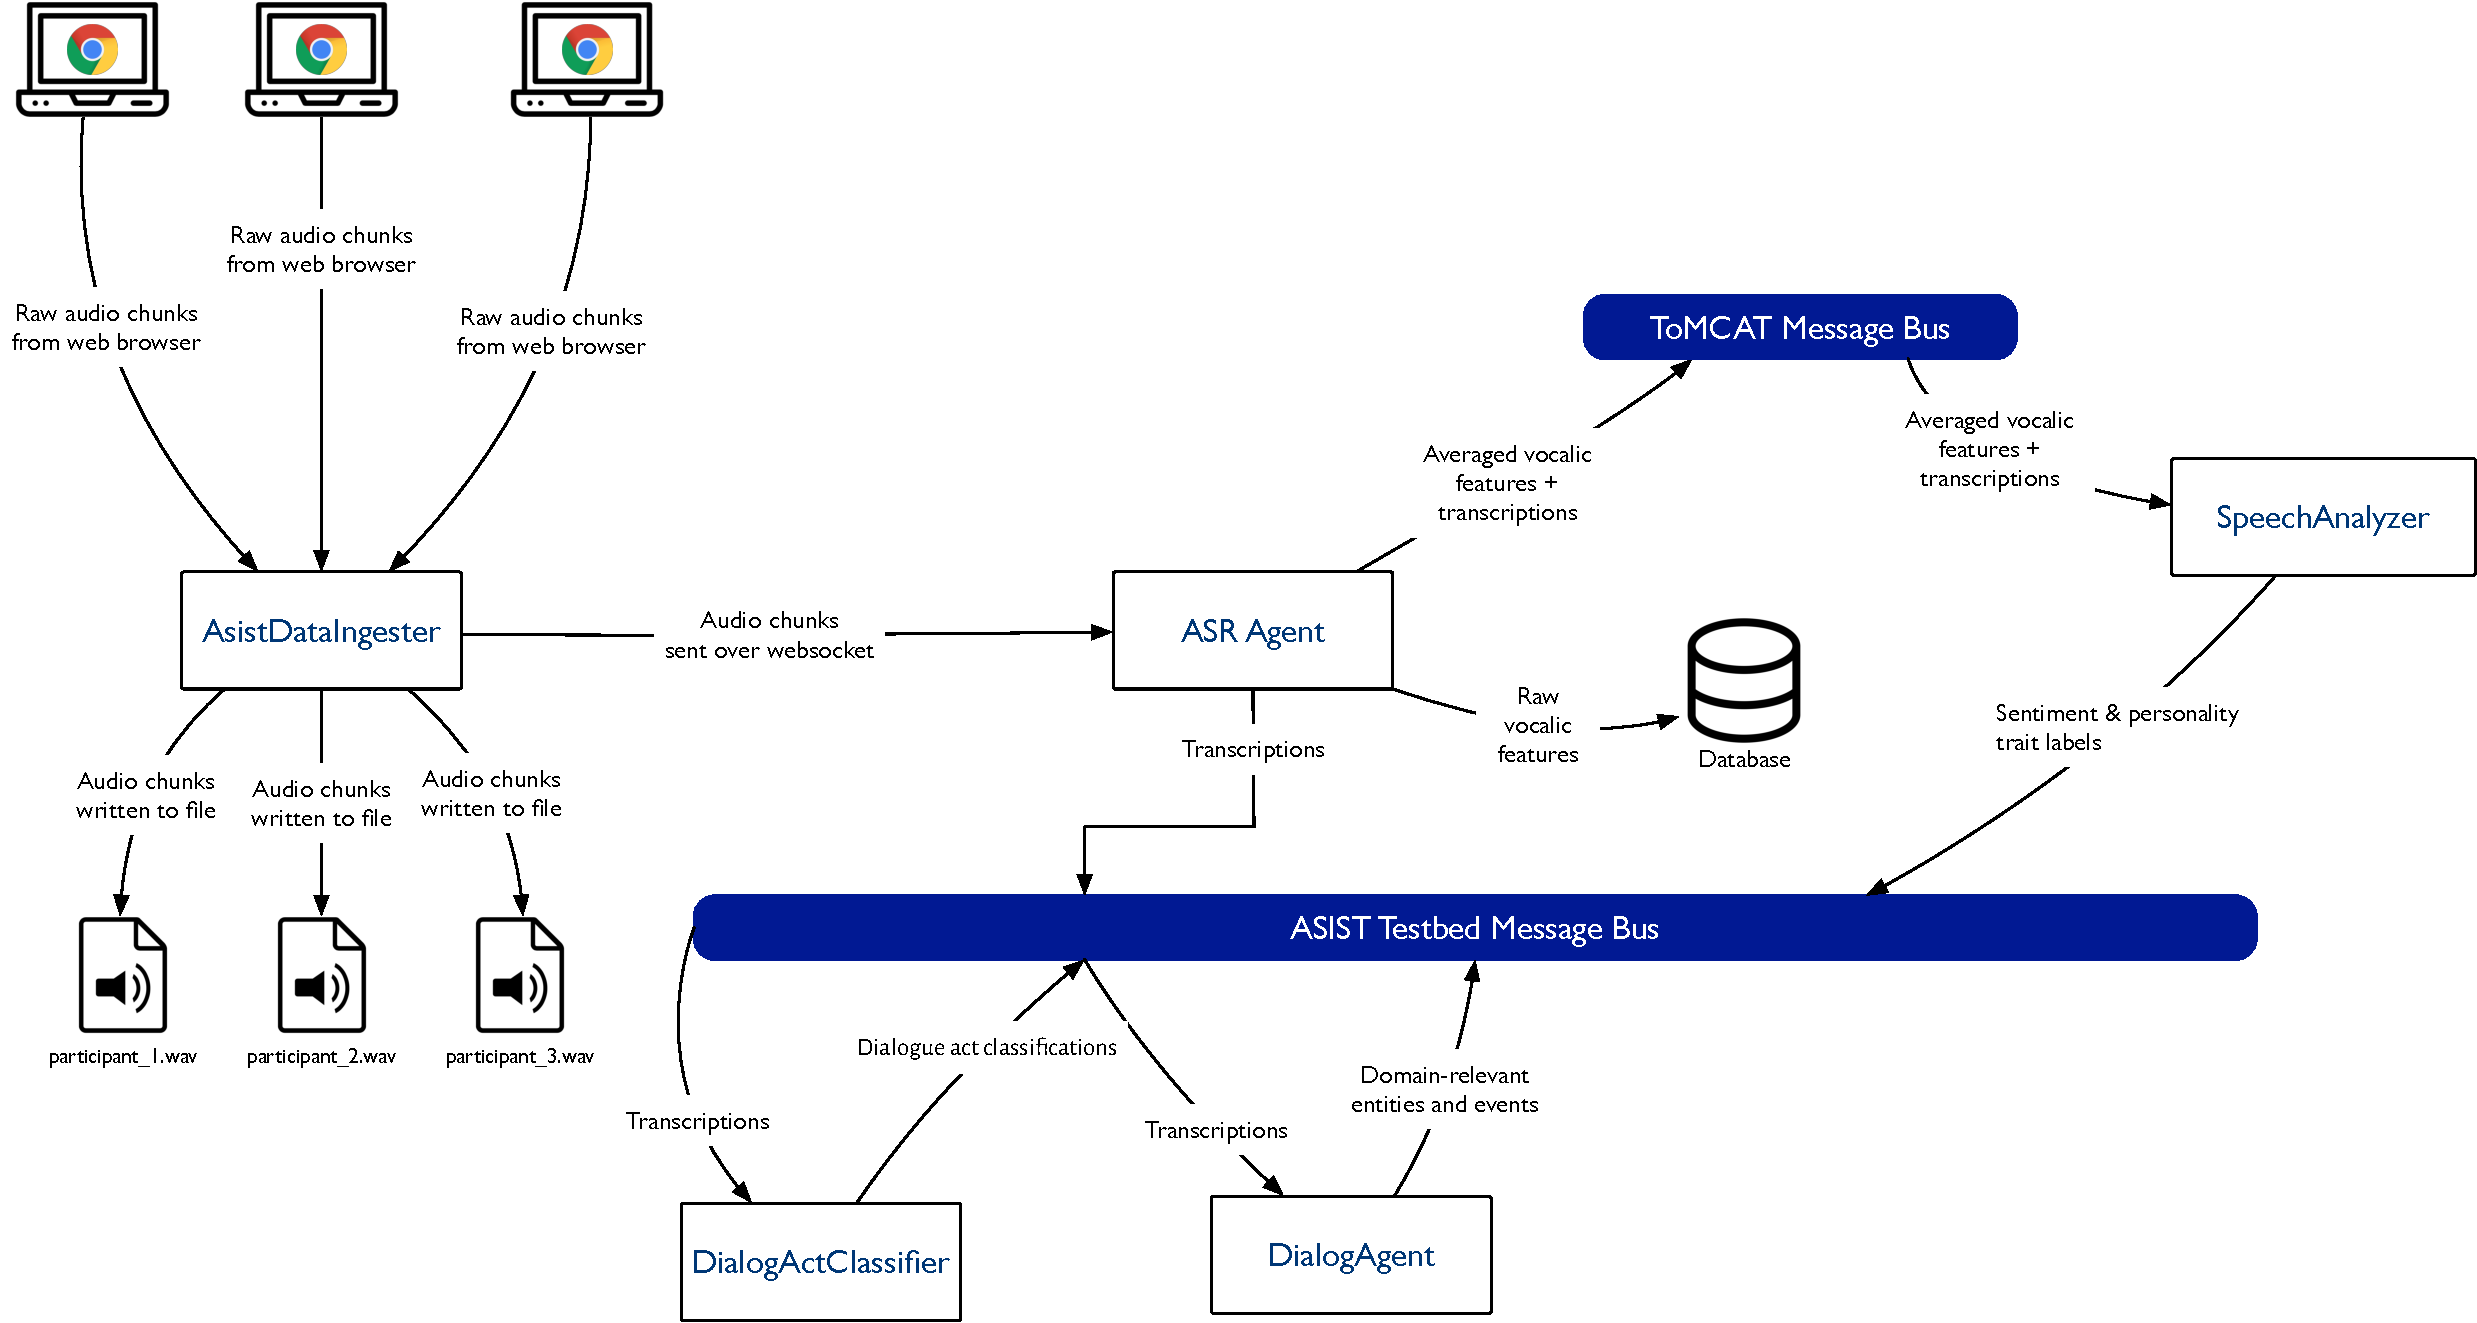
\includegraphics[width=6.5in]{images/nlp_architecture}
    \caption{Architecture of our multi-participant dialogue analysis system.}
\end{figure}

\chapter{Dialogue act classification}
\label{ch:da_classification}
\textbf{Ruihong Huang, Ayesha Qamar, Messal}

\section{Introduction}

In the Theory of Mind-based Cognitive Architecture for Teams (ToMCAT) project,
we are working on building an AI agent that will assist the players by taking
their speech and facial expressions as input. Speech being a core part of the
inputs, the agents will need to be capable of natural language understanding to
process the conversations to make informed and prompt decisions. Identifying
Dialog Acts (DA) is one of the primary aspects of natural language
understanding. dialog Act (DA) can be identified as a method of defining the
semantic content and communicative function of a single utterance of dialog
\citep{Searle:1969}. Examples include request, question, acknowledgment etc.
Dialog acts can provide important information about the user dialog turns and
set of possible system actions, and the frequencies and patterns of DAs spoken
by different speakers could also potentially indicate the roles they play such
as leader, follower etc., Thus, it is a useful capability for this AI agent and
many conversational agents in general.

Acknowledging the importance of DA classification in natural language
understanding, extensive research has been conducted on DA classification.
These research works have taken different approaches in terms of dataset,
machine learning model and input to the models. The most popular datasets that
are being used are Switchboard Corpus (SwDA) and ICSI Meeting Recorder Dialog
Act Corpus (MRDA). Most of the approaches use textual utterances from dialog
transcripts as input to the model. Statistical machine learning models such as
Support Vector Machines (SVMs) \citep{Henderson.ea:2012}, Hidden Markov Models
(HMMs) \citep{Stolcke.ea:2000}, Conditional Random Fields (CRFs)
\citep{Zimmermann:2009} are employed for identifying DAs. Deep learning models
are also gaining popularity in DA classification. \citet{Liu.ea:2017} presented
both CNN models and hierarchical CNN+CNN and CNN+RNN models to classify dialog
acts and showed that RNN/Bi-LSTM on top of CNN model performs better than other
models in consideration. \citet{Shen.ea:2016} presented that Neural Attention
Model with context information performed well on the SwDA dataset.
\citet{Raheja.ea:2019} achieved state-of-the-art result using context-aware
self-attention model on MRDA corpus. Another approach for DA classification is
incorporating both lexical and acoustic features. \citet{Ortega.ea:2018} showed
that their Lexico-Acoustic neural network models can outperform the similar
models taking only lexical information as input.

Even though these approaches provide excellent results on DA classification,
they lack in various aspects. First of all, most of these models require clean
transcripts as input. Achieving clean transcripts requires manual annotation,
which is both time consuming and costly. As a result, DA classification in real
time is not possible. Another limitation is the lack of explicit addressing to
multiparty dialogs where mechanisms to incorporate speaker identification and
determining the discourse structure is also crucial. Apart from these
limitations, these approaches often use only 5 types of high level tags for DA
classification, which do not entirely explain the DA under question. It is
necessary to have both general and specific tags to completely understand a DA.

We are going to develop a Deep neural network based DA classifier to process
the input utterances in real time which is more aligned with the main goal of
the project that is building an AI agent to be an effective teammate of a
Minecraft player. As the players will play online simultaneously, the agent
needs to understand the conversations of the player as the game progresses. For
the agent to be real time, we cannot rely on manual transcription. Instead we
have used a publicly available Automatic Speech Recognizer (ASR), named Google
Cloud Speech API to convert the utterances into text. This provides noisy text
in return which might harm the performance of the DA classifier. To compensate
for this, we will use acoustic features from the raw speech as well.

\section{Approach}
A Bi-LSTM based baseline model is already trained with clean transcripts. The
same model is trained again with the ASR generated transcripts and the
performance dropped significantly due to ASR noise and the highly overlapping
nature of the utterances in the meetings. To overcome this drop we will use a
fusion based audio-language model to leverage both lexical and acoustic
information of the utterances to successfully identify the DAs. In addition,
our approach will capture the threading structure within a dialogue that
involves detecting utterances falling within an adjacency pair (consisting of a
question and an answer utterance, or a request and an acceptance utterance) and
then linking them together. We will aim to eventually jointly learn both the
threading structure and DAs of a dialog in a multitask learning setting since
we expect the two tasks to benefit each other.

Currently we are using a multi-party dialog dataset MRDA
\citep{Shriberg.ea:2004} that consists of 75 meetings each about an hour long,
where each utterance has one (out of 11) general and zero or more (out of 40)
specific tags. Once the experimentation is done, we will use a transfer
learning approach to train and test the model for study-2 data. 

\section{Evaluation}

To evaluate our approach, we will use F1 score as the evaluation metric. For
multiclass classification problems, especially where the classes are highly
imbalanced, F1 score provides more insight than accuracy.  We also intend to
annotate ASIST data for dialog Acts so that the system trained on MRDA can be
finetuned on ASIST.

\chapter{Speech Analysis and Event Extraction}
\textbf{Remo Nitschke, Yuwei Wang}
\section{Introduction}

For humans, verbal and non-verbal communication are insightful indicators of social processes. Within the scope of ASIST, team-building and communication within teams is of heightened interest. We maintain, that in order to develop a model of human agents and human teams, surveying verbal communication is essential. Our DialogAgent is designed with this goal in mind: Extract information from player dialog that can be useful in order to create a model of the player's mental state.

An AI agent needs to formulate a model of the humans and teams it advises. In order to construct such a model, language data provides essential insights. As raw natural language data is ``messy", we believe it is necessary to pre-process and vet this data into chunks that are informative and pertinent to the AI. This is done via our DialogAgent which provides Dialog Act Labels and Event Extractions for player utterances. The Dialog Act Labels inform on the \emph{type} of utterance, whereas the Event Extractions inform on the semantic \emph{content} of the utterance. In this section we discuss the engine that constructs the Event Extractions.



\section{Approach}

%% Note to Adarsh: I think we could insert the diagram from Study 2 prereg here (page 2)

Raw communication audio captured during the experiments is processed through
our SpeechAnalyzer which provides transcriptions (transcriptions:
MinecraftEntity\_Observation\_Asr\_Speechanalyzer). The transcriptions are run through our DialogAgent which contains an extensive rule-based event extraction system (ODIN) \citep{valenzuela-escarcega-etal-2016-odins}. Much of modern information extraction and event extraction is done via neural nets, see \citet{Ahmad2021GATEGA,Du2020EventEB}. We are opting for a rule-based system because:

\begin{enumerate}
 \item It allows us to be more flexible with our extraction labels. We can quickly add or remove labels if we see the need to do so.
 \item It allows for high precision for the labels we are interested in. Rules can be crafted to be precise (albeit at the cost of coverage).
 \item Rules do not require us to create, maintain, and annotate extensive datasets. This is especially pertinent within the scope of ASIST, as domain specific terms can change between Studies. It would be near impossible for us to train a neural agent on the new terms of the next study before the data is published.
\end{enumerate}

Our rule based framework returns nested labels and their spans. The nesting of labels represents the argument structure of the event. The extracted events are returned as JSON objects (event extractions:MinecraftEntity\_Event\_Dialogue\_Event\_Dialogagent). 


%% Note to Adarsh: This is just a draft writeup if we want the IDC in the pre-reg:
%% Event extractions are then entered into a queue together with TAMU dialog act classifier labels for the utterance, player location data (location data: MinecraftEntity_Event_Location_Locationmonitor), victim triage status (triage status: MinecraftEntity_Event_Triage_Simulator), and rubble interactions (rubble interaction: MinecraftEntity_Event_Rubbledestroyed_Simulator). This queue feeds our InterdependenceAgent which aims to recognize interconnected utterances (speech acts), such as: players asking for help and other players providing said help, players negotiating plans, players responding negatively or positively to commands.

\subsection{List of Variables}
\begin{itemize}
    \item Input Variables
    \begin{itemize}
        \item transcriptions: MinecraftEntity\_Observation\_Asr\_Speechanalyzer
        %the following only if we want idc in pre reg:
        %\item location data: MinecraftEntity_Event_Location_Locationmonitor
        % \item triage status: MinecraftEntity_Event_Triage_Simulator
        %\item rubble interaction: MinecraftEntity_Event_Rubbledestroyed_Simulator
    \end{itemize}
    \item Output Variables
    \begin{itemize}
        \item Event Extractions: MinecraftEntity\_Event\_Dialogue\_Event\_Dialogagent
    \end{itemize}
\end{itemize}


\section{Evaluation}
We will evaluate via manual evaluation by human annotators. We will hire human annotators to evaluate a representative chunk of utterances. Annotators will receive transcripts with Event Extractions available for each utterance. We then ask them to evaluate whether the present Event Extraction Labels are precise and whether any labels are \emph{missing} in the Event Extractions. This way we can calculate precision and recall for a chunk of data, allowing us to calculate a representative F1 score.
We will also run a seperate evaluation for precision,\footnote{For reasons of economy, we restrict this evaluation to precision. Our expert team-members can judge produced labels for precision at a much higher speed than they can annotate utterances for labels.} done by team members who are familiar with our dialog agent labels.
\subsection{Potential Evaluation Problems}
There are two potential issues we may face with this mode of evaluation. 

Annotators may be primed by presence of extraction labels. If an annotator is asked to decide whether utterance X qualifies for label Y, they are more likely to assing label Y if the dialog agent already has done so. We could potentially avoid this effect by seperating the tasks of annotation and evaluation. Annotators are asked to only annotate and the evaluation is then done automatically by comparing label output of the dialog agent to the label output of the annotator. Here we run the risk of clerical errors by annotators muddying the data. Since the argument structure of our dialog agent labels can be quite complex, we believe that our proposed course of action is the lesser evil.

At time of writing the dialog agent contains 149 event labels it can assign. A possible risk of hired annotators is that they simply cannot reliably evaluate that number of labels. Even with a provided annotated list of labels (containing small descriptions), we will have to assume that some false negatives\footnote{Due to the setup, we anticipate very few false positives and a larger amount of false negatives in the human evaluation. We assume that it is easier for an annotator to review whether a complex label is correct than to assign a complex label where none is given.} will occur. For this reason, we will run a seperate evaluation for precision only, done by expert members of the team who should have high familiarity with our labels.

\chapter{Sentiment analysis and personality trait detection}
\textbf{John Culnan}
\section{Introduction}
\begin{itemize}
    \item Why is this a useful capability for an AI
        agent? How does it contribute to machine theory of mind/machine theory
        of teams?
    \item What are the existing state of the art approaches to this problem
        (cite relevant papers including \textcite{culnan-etal-2021-ire}), and
        what are their limitations? 
    \item What is our approach, and how will it address those limitations?
\end{itemize}

\section{Approach}
\begin{itemize}
    \item Provide details on our approach, including:
        \begin{itemize}
            \item What data is required for this work? If any of the required
                inputs are present in the table of Study 3 variables in the
                \href{https://docs.google.com/document/d/1GF7VsNF9R95IAaj6mVZUDV2mAX5ok1Bh6Tcm8zDpIkg/edit#heading=h.1ksv4uv}{TA3
                Study 3 preregistration document (table 3)}, please list those
                variables with the standardized verbose variable names in the table.
        \end{itemize}
\end{itemize}

\section{Evaluation}
\begin{itemize}
    \item How will we evaluate our approach?
\end{itemize}

\chapter{Entrainment detection}
\label{ch:entrainment}

\textbf{Meghavarshini Krishnaswamy, Andrew Wedel, Adam Ussishkin, Cheonkam Jeong} 
\section{Introduction}

    Entrainment (also referred to as `synchronization', `coordination', or `alignment') is the adaption of verbal and non-verbal actions by conversation partners to more closely resemble one another \parencite{borrie2014}. Its role in communication as been described as ``key for supporting important pragmatic aspects of conversation, including taking turns, interaction smoothness, building rapport, fostering social bonds, and maintaining interpersonal relationships''\parencite{borrie2019}. A time-sensitive cooperative task utilizing verbal communication would require participants to optimize their information channel. This makes entrainment a useful metric for assessing the degree of cooperation among teammates, as well as a useful means to assess members' sentiments towards each other, tracking their confidence in the task goals and plans, and identifying team cohesion and bonding over time.

    In speech, entrainment has been observed and analysed using speech rhythm and
    timing, pitch, MFCCs and formant analysis \parencite{reichel2018prosodic,borrie2019syncing}. Speech entrainment occurs in correlation with entrainment at other linguistic levels such as an increase in shared vocabulary and sentence structures \parencite{rahimi2017entrainment}. While entrainment in multi-party conversations has been researched at the lexical-level and sentence-level, speech entrainment has mostly been restricted to two-party conversations. Work on speech entrainment is further limited by the practical difficulties in identifying speech similarity due to the process of entrainment from similarities from physical factors such as people having similar vocal characteristics, or sharing the same speech channel \parencite{nasir2020}.

    Recent research on vocal entrainment has shifted from regression-based analysis to encoding-based neural networks for a few reasons: to model the non-linear relationship between vocalic features, to capture the complexity and diversity of both entrainment and disentrainment, and to train the model on information relevant to entrainment, while ignoring other factors that cause similarity (such as speaker characteristics and features related to the speech recording channel)\parencite{nasir2020}.


\section{Approach}
    The main assumption for automated entrainment detection is that for a given set of speakers and utterances in a discourse, if entrainment takes place, it is located between two neighbouring utterances from different speakers, while utterances from different time points will not show entrainment. So, the model needs to correctly identify neighbouring pairs of utterances, while ignoring similarities pertaining to speaker and channel characteristics (since they are not a function of entrainment). For a multi-party conversation setting, the model also needs to tell the difference between a pair of entrained utterances, a pair of utterances from the same speaker, and utterances from different speakers that are not neighbours.

    Our approach involves training an replicating the feed-forward encoder model and i-vector modelling for entrainment detection proposed and designed by \citeauthor{nasir2020}. This model assess triplets of utterances for each speaker arranged as follows: an utterance by a given speaker, the utterance succeeding it spoken by a different speaker (positive match for entrainment), and an utterance from a different location in the discourse uttered by the given speaker (negative match for entrainment). In the training process, positive weights are assigned to entrainment characteristics, while speaker and channel characteristics are assigned negative weights. We thus have a classification task in which for a given pair of utterances, we ask if one is the entrainment pair of the other or not.

    \begin{figure}
    \begin{sidecaption}{Representation of the triplet model proposed by \citeauthor{nasir2020}[Pg17]. Here, ``Speaker 1 (anchor)'' and `Speaker 2 (positive)' refer to the site of entrainment, while `negative' refers to a non-entrainment utterance}
    \centering
    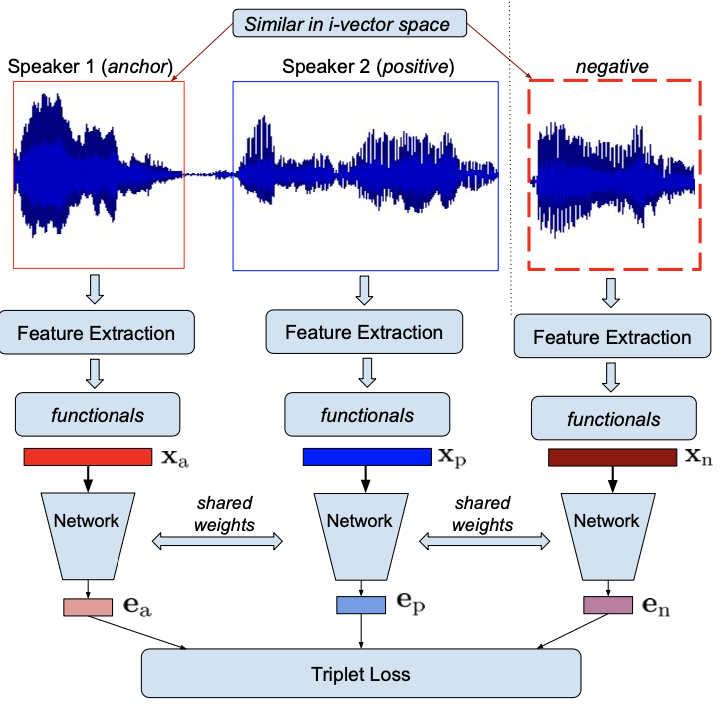
\includegraphics[width=0.6\textwidth]{images/triplet-model.png}
    \label{fig:sentiment_model_schematics}
    \end{sidecaption}
    \end{figure}

    We will utilize the following data and labels from Study-3-
            \begin{itemize}               
                   \item Audio recording
                    Transcript
                   \item Participant demographic information
                   \item Self-evaluation
                   \item MinecraftEntity\_Observation\_Asr\_Speechanalyzer
                   \item MinecraftEntity\_Observation\_Audio\_Speechanalyzer
                   \item MinecraftEntity\_Event\_Dialogue\_Event\_Dialogagent
            \end{itemize}
        % \item Our objectives (in decreasing order of priority):
        %     \begin{itemize} 
        %         \item Build a working statistical model for assessing entrainment while utilizing the vocalic features extracted by the ToMCAT-speechanalyzer system.         
        %         \item Train an encoding-based model using the methodology outlined in \textcite{nasir2020} for a simple classification task that identifies entrainment and directionality in a given conversation.
        %         \item Assess if the current Speechanalyzer system is set up to study entrainment trends as a time series. 
        %     \end{itemize} 

\section{Evaluation}

    Assessing entrainment involves calculating a similarity (or dissimilarity) measure between two utterances from the entrainment category, and to observe if this metric of similarity increases or decreases as the speakers continue communicating. For this objective, accuracy scores for the classification task outlined above will be used to measure the performance of the entrainment detector. Because ASIST-ToMCAT is a multi-party conversation, we will examine the process of setting up new baselines for entrainment detection that can account for differences in team dynamics, reflected in how much each speaker talks, and how much other speakers respond to them.  

    We will also explore methods to evaluate two types of entrainment:

    \begin{itemize}
        \item Localized entrainment: Are there observable similarities between utterances by different speakers that occurred next to each other than utterances at different points in time?
        \item Global entrainment: after a given period of objective-oriented speech, is the speech from the conversation aligned more closely? 
    \end{itemize}

    In order to account for ASR errors in the automatically generated transcripts, we will create a corpus of human-generated gold transcriptions. From this corpus, a subsection of the data will be used to identify utterances separated by 50ms pauses; in order to assess any differences in performances due to ASR issues. A manual evaluation of the speech data will also be conducted to examine other environmental noise, so as to account for qualitative differences between the recording conditions of the pristine training data and the real-time ToMCAT speech data. 

   \section{Other Qualitative Assessments}

   Since speech entrainment in conversational setups is a feature of speaker bonding and closeness, it is useful to assess if it co-occurs with positive emotions in spoken statements, lower stress, and higher confidence in the plan and team actions in a co-operative goal-oriented setting. We will utilise the human-generated gold transcriptions as well as manual annotations for emotion and dialogue acts to qualitatively assess if entrainment co-occurs with positive emotions and the acts of sharing information, as well as the relationship between global entrainment and levels of stress and uncertainty. We will also examine if the directionality of entrainment (towards or away from any of the participants) is affected by members' personality or socio-cultural differences, in order to account for natural differences known to impact conversation styles.


\chapter{Online multi-agent plan recognition}
\label{ch:plan_recognition}
\textbf{Loren Champlin, Salena Ashton, Liang Zhang, Clayton Morrison}

\section{Introduction}

Plan recognition is the ability to understand and recognize logical structures
and patterns within a sequence of observed behavior. Developing this capability
for our AI agent would allow it to infer the latent plan structures,
strategies, and goals (i.e., `plan explanations') of not only individual human
agents but a team of agents as well. Producing these plan explanations
contributes to the logical belief structures that the AI agent must maintain as
part of its theory of mind and theory of teams
\citep{Tambe_1997,Baker_Tenenbaum_2014}. Furthermore, an AI agent could use
these inferred plan explanations to predict the teams' subsequent actions and
to help develop potential interventions for increasing team performance. Our AI
agent must recognize the conjoined plan explanations of multiple agents given
our team search and rescue setting and demonstrate this capability online
(i.e., as the team carries out their mission). While a highly sparse topic,
there are a few existing "state of the art" approaches for online Multi-Agent
Plan Recognition (MAPR). 

The most recent online MAPR approach by \citet{Argenta_Doyle_2017} uses an automated planner to produce feasible plan explanations by simulating potential sets of parameters, conditions, and plan structures needed to generate the observed behavior. Approaches of this type are known as \textit{plan recognition as planning approaches} \citep{Ramirez_Geffner_2009,Van-Horenbeke_Peer_2021}. The use of an automated planner requires constructing a symbolic representation of the problem domain in which MAPR is to be deployed, known as knowledge engineering. Plan recognition as planning approaches are typically highly expressive and are capable of solving plan recognition problems that involve high levels of logical reasoning. However, this high expressivity usually comes at the cost of the high computational complexity required by the automated planner \citep{Van-Horenbeke_Peer_2021}. \citet{Argenta_Doyle_2017} attempt to overcome this challenge by making several strict simplifying assumptions about their problem domain. Although, these assumptions reduce the computational complexity at the cost of expressivity (i.e., it limits the type of problems their approach can solve). Another limitation is that \citet{Argenta_Doyle_2017} only consider ``flat" knowledge representations, rendering their approach incapable of inferring more than just the end-goals that the agents are trying to achieve. However, human behavior tends to exhibit hierarchical structures or patterns such that simple actions are combined to produce more complex actions. In terms of having a complete theory of mind and theory of teams, an AI agent needs to understand how actions relate to each other at different levels of granularity and complexity, not just how they relate to the agents' end-goals. 

Our proposed method for online MAPR is also a \textit{plan recognition as planning} approach. Rather than make assumptions that limit the problems our approach can solve, we try to overcome the challenges of computational complexity by developing a highly efficient automated planning algorithm specialized towards doing online MAPR. Our automated planning algorithm combines the well-known Simple Hierarchical Ordered Planner (SHOP2) proposed by \citet{Nau_2003} and the Monte Carlos Tree Search (MCTS) single-agent plan recognition algorithm proposed by \citet{Kantharaju_Ontanon_Geib_2019}. We also draw heavy inspiration from known parsing algorithms for Probabilistic Context-Free Grammars (PCFG) \citep{Collins_2011}. As suggested by its partial adaption of the SHOP2 algorithm, our approach assumes that the agents' actions relate through a set of hierarchical structures or what is known as a hierarchical task network (HTN) \citep{Nau_2003,Russell_Norvig_2021}. As such, our approach produces the most likely task hierarchy, which is an instance of a HTN under specific initial conditions. These task hierarchies represent how actions relate to each other at different levels of granularity of complexity by showing how high-level actions (also known as compound tasks) can be decomposed into low-level actions. 

\section{Approach}
In a HTN domain representation, compound tasks are high-level actions that are
composed of lower-level actions. These lower-level actions may be compound task
themselves that need to be further decomposed or non-decomposable actions,
which are sometimes referred to as primitive tasks or just actions
\citep{Russell_Norvig_2021}. Depending on how abstractly a compound task is
defined, there may be multiple sets of lower-level actions that could be
combined to create the same compound task. These different sets of actions are
known as ``methods", since they are different ways of decomposing the compound
task \citep{Russell_Norvig_2021}. Additionally, methods typically have
preconditions, which are specific conditions that must be satisfied by the
current state of the problem domain for that method to be used for task
decomposition. If a methods preconditions are satisfied, then that method is
said to be applicable \citep{Russell_Norvig_2021}. \autoref{fig:pr1} further illustrates the concepts of compound tasks, actions, methods, and task decomposition. In the illustration, both methods could applicable or only one of them could be applicable given the current state of the problem domain. In the former case, an automated planner must choose one of the methods for decomposition, leading to two different possible plans. Further details on HTN planning processes can be found in the automated planning literature. (e.g., the SHOP2 paper by \citet{Nau_2003}). 

\begin{figure}
    \centering
    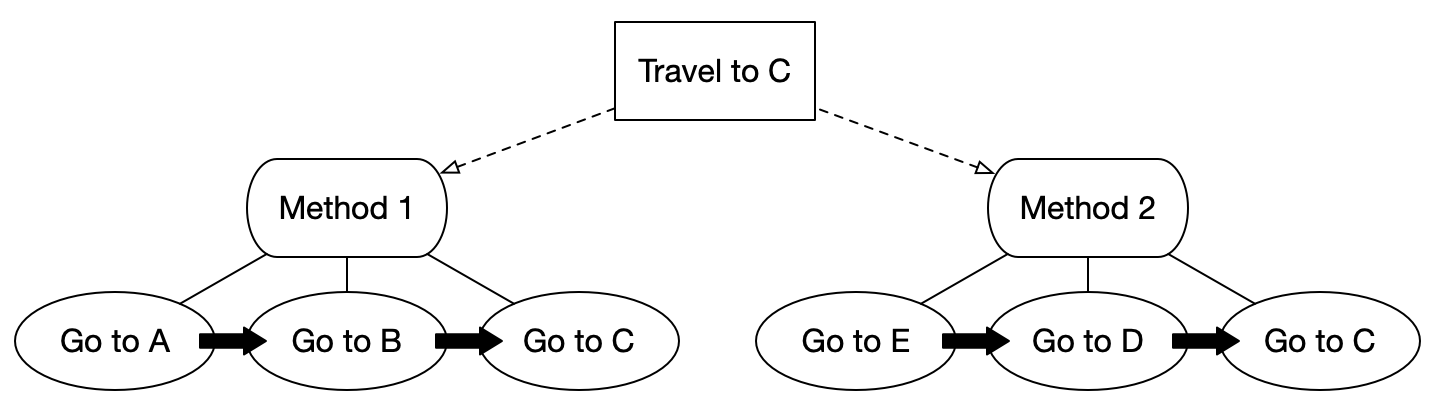
\includegraphics[width=\textwidth]{../images/htn_concepts}
    \caption{The compound task \textit{Travel to C} is shown to have two different methods for accomplishing the same task.} 
    \label{fig:pr1}
\end{figure}

Our approach uses a HTN domain representation and an automated HTN planner to
model the logical reasoning and decision-making process of a team of human
agents. Compound tasks and methods are engineered in such a way as to represent
the latent decisions that agents must make to complete their mission. From a
generative perspective, these latent decisions are then what leads to the
actions we observe from the human agents. With this concept in mind, we can
have an automated planner generate a plan that matches the observed actions
while recording the methods and task decompositions involved. As suggested in
the introduction, this record is produced in the form of a task hierarchy which
shows how compound task can be decomposed into the actions we observe. These
task hierarchies are the plan explanations that give insight on the
relationship between actions and the decision-making process of the agents.
\autoref{fig:pr2} illustrates the general concept of our online MAPR approach.

\begin{figure}
    \centering
    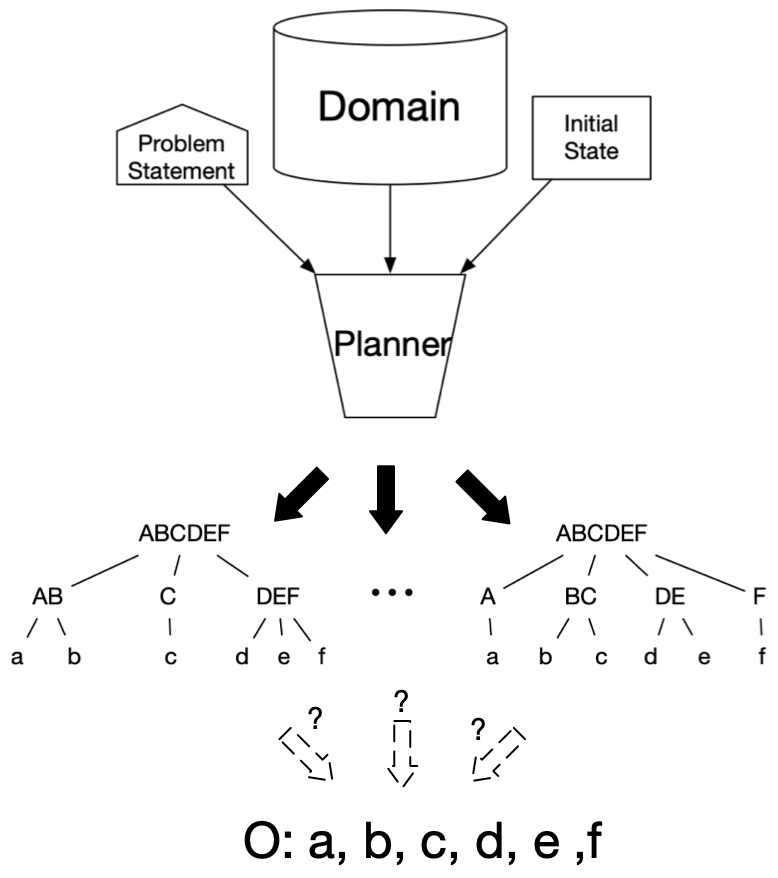
\includegraphics[width=\textwidth]{../images/pr_as_planning}
    \caption{In this illustration compound task are represented as groups of upper-case letters and actions are singular lower-case letters. Multiple potential task hierarchies can be generated for the same observed plan.} 
    \label{fig:pr2}
\end{figure}

As seen in  \autoref{fig:pr2}, it is possible that there are multiple plan explanations for same observed actions. However, rather than obtain all potential plan explanations given an observed sequence of actions, our approach should be yielding the most likely plan explanation. With this in mind, our approach assigns a conditional probability $p(m | \bigcap_{n \in M_t} c_n(s), s)$ for a method $m \in M_t$ for a compound task $t$. $c_n(s)$ denotes a function that is 1 if $n \in M_t$ is applicable to $t$ for the current state $s$, and 0 otherwise. The conditional probabilities are then defined as,

\begin{equation} \label{pr_eq:1}
p(m | \bigcap_{n \in M_t} c_n(s), s) = \begin{cases} \alpha  & c_m(s) = 1 \\ 0 & c_m(s) = 0 \\ \end{cases}
\end{equation}

\begin{equation}  \label{pr_eq:2}
\sum_{m \in M_t} p(m | \bigcap_{n \in M_t} c_n(s), s) = 1
\end{equation}

The value denoted by $\alpha$ in (\ref{pr_eq:1}) of each conditional probability must be predefined. As part of our approach we have formulated a training algorithm for learning these conditional probabilities, however that training algorithm is not detailed here. 

As suggested, an automated planner uses the methods defined in a HTN domain representation to decompose a compound task or set of compound tasks into a plan. This derivation of a plan is an analogous process to deriving a sentence from a PCFG. A PCFG contains a vocabulary of both non-terminal symbols and terminal symbols, as well as a set of derivation rules for replacing non-terminal symbols with a sequence of both non-terminal and terminal symbols \citep{Collins_2011}. Given an initial non-terminal symbol and applying rules successively eventually yields a sequence of only terminal symbols (i.e., a sentence) \citep{Collins_2011}. Similar to the methods of our HTN domain representation, each derivation rule is assigned a probability. Thus, given a specific derivation of a sentence (i.e., a specific set of derivations rules used), the probability of that derivation is the product of the probabilities of each rule used \citep{Collins_2011}. Given the similarities, we define the probability of a specific task hierarchy for a given plan in the same way. We denote $m_t$ as the applicable method chosen to decompose task $t \in \tau_\pi$, where $\tau_\pi$ is a set of tasks representing some task hierarchy used to generate a plan $\pi$. Using (\ref{pr_eq:1}), we have that,

\begin{equation} \label{pr_eq:3}
p(\tau_\pi) = \prod_{t \in \tau_\pi} p(m_t | \bigcap_{n \in M_t} c_n(s_t), s_t) 
\end{equation}

$s_t$ is current state prior to the decomposition of task $t$. Since our approach is for online MAPR, we want our plan explanations to consist of a partial task hierarchy that shows how the agents' latent decisions generates their plans up to the current time step. We denote the agents' observed partial plan (i.e., their observed sequence of actions up to some current time step) as $\pi^*$. We then simply replace $\pi$ in (\ref{pr_eq:3}) with $\pi^*$ to get,

\begin{equation} \label{pr_eq:4}
p(\tau_{\pi^*}) = \prod_{t \in \tau_{\pi^*}} p(m_t | \bigcap_{n \in M_t} c_n(s_t), s_t) 
\end{equation}

Using (\ref{pr_eq:4}), the objective of our approach is then to compute 

\begin{equation} \label{pr_eq:5}
\hat{\tau}_{\pi^*} = \argmax_{\tau_{\pi^*} \in T_{\pi^*}} p(\tau_{\pi^*})
\end{equation}

In (\ref{pr_eq:5}), $T_{\pi^*}$ denotes the set of all partial task hierarchies that match the observed partial plan $\pi^*$.

SHOP2 uses a depth first search (DFS) algorithm to generate plans and as such we could modify it to generate $T_{\pi^*}$ and then compute $\hat{\tau}_{\pi^*}$ by comparing $p(\tau_{\pi^*})$ for all $\tau_{\pi^*} \in T_{\pi^*}$ \citep{Nau_2003}. This is however an extremely computationally complex procedure and not a feasible method, especially for online MAPR where we would need to run this same computation many times. In general, using any automated planning algorithm to generate $T_{\pi^*}$ is not feasible. 

We argue that reasonable method would be to instead sample partial task hierarchies from $T_{\pi^*}$ and estimate $\hat{\tau}_{\pi^*}$ instead, this estimate being denoted $\bar{\tau}_{\pi^*}$. \citet{Kantharaju_Ontanon_Geib_2019} had come to this same conclusion in their development of an approach to do single-agent plan recognition using a domain representation based on Combinatory Categorical Grammars (CCGs). As mentioned in the introduction, they use a MCTS algorithm to sample the space of plans and find a reasonable estimate of the most likely plan explanation for an observed plan, reducing the computational complexity of their approach significantly. Using a similar concept, we modified the SHOP2 algorithm to use a MCTS algorithm as opposed to DFS. Although we will not go into full details here, MCTS samples solutions from the search space, which in our case are partial plan hierarchies matching the agents' observed partial plans. The search algorithm uses each sample to compute statistics about the search space that inform it where ``good" areas of the search space are according to some utility function \citep{Browne_Powley_Whitehouse_Lucas_Cowling_Rohlfshagen_Tavener_Perez_Samothrakis_Colton_2012,Kantharaju_Ontanon_Geib_2019}.In our case, our utility function is $p(\tau_{\pi^*})$, which the algorithm attempts to maximize. MCTS balances its search between completely unexplored areas and areas of the search space that have yielded good results before \citep{Browne_Powley_Whitehouse_Lucas_Cowling_Rohlfshagen_Tavener_Perez_Samothrakis_Colton_2012,Kantharaju_Ontanon_Geib_2019}. Given enough search time, our MCTS algorithm will eventually compute $\hat{\tau}_{\pi^*}$, although the needed search time would be roughly equivalent to what SHOP2 would need to do the same task. Therefore we must limit the search time allowed and have our algorithm return the best $\tau_{\pi^*}$ it can find under a predefined search time, which is our estimate $\bar{\tau}_{\pi^*}$. There is a high chance that $\bar{\tau}_{\pi^*}$ may only be a local optima, but it is likely to be a sufficiently probable plan explanation given a reasonable amount of search time. 

In terms of the Study 3 data, our approach heavily utilizes the json mission event messages coming from the message bus during the Search and Rescue mission trials. These messages are primarily used as the observations for our plan recognition algorithm, but are also used along with the video of the trials as source material for knowledge engineering our HTN domain representation. We also use the messages in our training algorithm to learn the conditional probabilities as defined in \ref{pr_eq:1} and \ref{pr_eq:2}. The specific input variables that we use in our approach from the message bus are as followed, 

\begin{itemize}
\item MinecraftEntity\_Event\_Triage\_Simulator
\item MinecraftEntity\_Event\_Roleselected\_Simulator
\item MinecraftEntity\_Event\_Proximityvictiminteraction\_Simulator
\item MinecraftEntity\_Event\_Playerfrozenstatechange\_Simulator
\item MinecraftEntity\_Event\_Tooldepleted\_Simulator
\item MinecraftEntity\_Event\_Markerplaced\_Simulator
\item MinecraftEntity\_Event\_Markerremoved\_Simulator
\item MinecraftEntity\_Event\_Markerdestroyed\_Simulator
\item MinecraftEntity\_Event\_Victimpickedup\_Simulator
\item MinecraftEntity\_Event\_Victimplaced\_Simulator
\item MinecraftEntity\_Event\_Rubbleplaced\_Simulator
\item MinecraftEntity\_Event\_Rubbledestroyed\_Simulator
\item MinecraftEntity\_Event\_Victimnolongersafe\_Simulator
\item MinecraftEntity\_Event\_Missionstate\_Simulator
\item MinecraftEntity\_Event\_Location\_Locationmonitor
\item MinecraftEntity\_Event\_Victimsexpired\_Simulator
\item MinecraftEntity\_Observation\_State\_Simulator
\item MinecraftEntity\_Observation\_Fov\_Fovtool
\item MinecraftEntity\_Event\_Dialogue\_Event\_Dialogagent
\end{itemize}

\section{Evaluation}
Since it would be extremely difficult to objectively confirm a teams latent decision process used for a mission trial, we have devised an alternative evaluation method for testing the performance of our online MAPR approach. The algorithm described in our approach section, can be reconfigured to project forward in time past the agents' observed partial plan, effectively allowing it to predict their most probable next actions using $\bar{\tau}_{\pi^*}$ as a reference point for the agents' latent decision-making process. We reason that the closer $\bar{\tau}_{\pi^*}$ is to the true value, the more accurate the action prediction will be. Using this concept, we can indirectly measure how well our approach works by measuring how accurate the action predictions are given $\bar{\tau}_{\pi^*}$.

While our algorithm could technically project forward to the end of a team's mission trial, we expect the prediction accuracy to increasingly diminish as the gap between the end of the projected plan and the observed partial plan increases. Instead we evaluate our algorithms performance by having it use $\bar{\tau}_{\pi^*}$ to predict only the next few actions. Given an observed plan from a completed mission trial, we can simulate having a teams' observed partial plan at a set time points in their mission. At these set time points, we can run our online MAPR algorithm and then have our planner predict the next few actions, and compare these predicted actions against the teams' true actions. 

We will compute two different types of accuracy measures, the action allocation accuracy and the action sequence accuracy, which are accuracy measures used in other MAPR literature \citep{Kim_Chacha_Shah_2015}. The action allocation accuracy is the ratio of how many predicted actions were correct out of the number of actions predicted \citep{Kim_Chacha_Shah_2015}. The action sequence accuracy is computed by first dividing the correctly predicted actions into pairs and then counting how many pairs are in the correct order (regardless of what actions they are predicted to have between them). This count is divided by what the count would be if all pairs were correctly ordered \citep{Kim_Chacha_Shah_2015}. The average action allocation and average action sequence accuracy over all trials will be computed for each prediction point, as well as average accuracy measures over all prediction points over all trials. 

We will also measure the rate at which our prediction accuracies decrease as we increase the number of actions predicted. This can be done by picking a singular prediction point for each trial and measuring the action allocation accuracy and action sequence accuracy as we increase the number of actions predicted. Increases in te number of actions predicted will be done at set intervals (e.g., 2 actions, 4 actions, 6 actions, etc).  Average accuracies will then be computed for each interval over all trials. 

\chapter{Probabilistic modeling of team dynamics}
\textbf{Paulo Soares, Kobus Barnard, Emily Butler}
\section{Introduction}
\begin{itemize}
    \item Why is this a useful capability for an AI
        agent? How does it contribute to machine theory of mind/machine theory
        of teams?
    \item What are the existing state of the art approaches to this problem
        (cite relevant papers), and what are their limitations? 
    \item What is our approach, and how will it address those limitations?
\end{itemize}

\section{Approach}
\begin{itemize}
    \item Provide details on our approach, including:
        \begin{itemize}
            \item What data is required for this work? If any of the required
                inputs are present in the table of Study 3 variables in the
                \href{https://docs.google.com/document/d/1GF7VsNF9R95IAaj6mVZUDV2mAX5ok1Bh6Tcm8zDpIkg/edit#heading=h.1ksv4uv}{TA3
                Study 3 preregistration document (table 3)}, please list those
                variables with the standardized verbose variable names in the table.
            \item What interventions will we be testing and why?
        \end{itemize}
\end{itemize}

\section{Evaluation}
\begin{itemize}
    \item How will we evaluate our approach?
\end{itemize}


% hypotheses?
% - TMM model can predict behavior
% - TMM agent interventions improve performance
% - Closed loop communication is predictive of team performance
\printbibliography
\end{document}
